%-----------------------------------------
% Note: Use pdflatex to process this file.
%-----------------------------------------

%\documentclass{article}
\documentclass{hitec}

\usepackage{setspace}
\usepackage{graphicx}
\usepackage{moreverb}    % Defines {listing} environment.
\usepackage{amsmath, amsthm, amssymb, amsbsy, mathtools}
\usepackage{alltt}
\usepackage{rotating}
\usepackage[TABBOTCAP]{subfigure}
\usepackage{toc-bmad}
\usepackage{xspace}
%%\usepackage{makeidx}
\usepackage[section]{placeins}   % For preventing floats from floating to end of chapter.
\usepackage{longtable}  % For splitting long vertical tables into pieces
\usepackage{index}
\usepackage{multirow}
\usepackage{booktabs}   % For table layouts
\usepackage{yhmath}     % For widehat

\usepackage[T1]{fontenc}   % so _, <, and > print correctly in text.
\usepackage[strings]{underscore}    % to use "_" in text
\usepackage[pdftex,colorlinks=true]{hyperref}   % Must be last package!

%----------------------------------------------------------------

\newcommand{\extref}[1]{$\S$\ref*{#1}}   % No hyperlink. For external refs. \extref
\newcommand{\comma}{\> ,}
\newcommand{\period}{\> .}
\newcommand{\wt}{\widetilde}
\newcommand{\grv}{\textasciigrave}
\newcommand{\hyperbf}[1]{\textbf{\hyperpage{#1}}}
\newcommand{\Ss}{\(^*\)}
\newcommand{\Dd}{\(^\dagger\)}

\newcommand{\AND}{&& \hskip -17pt\relax}
\newcommand{\CR}{\\}
\newcommand{\CRNO}{\nonumber \\}
\newcommand{\dstyle}{\displaystyle}

\newcommand{\Begineq}{\begin{equation}}
\newcommand{\Endeq}{\end{equation}}
\newcommand{\NoPrint}[1]{}

\newcommand{\pow}[1]{\cdot 10^{#1}}
\newcommand{\Bf}[1]{{\bf #1}}
\newcommand{\bfr}{\Bf r}

\newcommand{\bmad}{{\sl Bmad}\xspace}
\newcommand{\tao}{{\sl Tao}\xspace}
\newcommand{\mad}{{\sl MAD}\xspace}
\newcommand{\cesr}{{\sl CESR}\xspace}

\newcommand{\sref}[1]{\S\ref{#1}}
\newcommand{\Sref}[1]{Sec.~\sref{#1}}
\newcommand{\cref}[1]{Chapter~\ref{#1}}

\newcommand{\Newline}{\hfil \\ \relax}

\newcommand{\eq}[1]{{(\protect\ref{#1})}}
\newcommand{\Eq}[1]{{Eq.~(\protect\ref{#1})}}
\newcommand{\Eqs}[1]{{Eqs.~(\protect\ref{#1})}}

\newcommand{\vn}{\ttcmd}           % For variable names
\newcommand{\vni}{\ttcmdindx}
\newcommand{\cs}{\ttcmd}           % For code source
\newcommand{\cmd}{\ttcmd}          % For Unix commands
\newcommand{\rn}{\ttcmd}           % For Routine names
\newcommand{\tn}{\ttcmd}           % For Type (structure) names
\newcommand{\bn}[1]{{\bf #1}}       
\newcommand{\toffset}{\vskip 0.01in}
\newcommand{\rot}[1]{\begin{rotate}{-45}#1\end{rotate}}

\newcommand{\data}{{\mbox{data}}}
\newcommand{\reference}{{\mbox{ref}}}
\newcommand{\model}{{\mbox{model}}}
\newcommand{\base}{{\mbox{base}}}
\newcommand{\design}{{\mbox{design}}}
\newcommand{\meas}{{\mbox{meas}}}
\newcommand{\var}{{\mbox{var}}}

\newcommand\ttcmd{\begingroup\catcode`\_=11 \catcode`\%=11 \dottcmd}
\newcommand\dottcmd[1]{\texttt{#1}\endgroup}

\newcommand\ttcmdindx{\begingroup\catcode`\_=11 \catcode`\%=11 \dottcmdindx}
\newcommand\dottcmdindx[1]{\texttt{#1}\endgroup\index{#1}}

\newcommand{\St}{$^{st}$\xspace}
\newcommand{\Nd}{$^{nd}$\xspace}
\newcommand{\Th}{$^{th}$\xspace}
\newcommand{\B}{$\backslash$}
\newcommand{\W}{$^\wedge$}

\newcommand{\cbar}[1]{\overline C_{#1}}

\newlength{\dPar}
\setlength{\dPar}{1.5ex}

\newenvironment{example}
  {\vspace{-3.0ex} \begin{alltt}}
  {\end{alltt} \vspace{-2.5ex}}

\newcommand\Strut{\rule[-2ex]{0mm}{6ex}}

\newenvironment{Itemize}
  {\begin{list}{$\bullet$}
    {\addtolength{\topsep}{-1.5ex} 
     \addtolength{\itemsep}{-1ex}
    }
  }
  {\end{list} \vspace*{1ex}}

\newcommand{\Section}[1]{\section{#1}\indent\vspace{-3ex}}

\newcommand{\SECTION}[1]{\section*{#1}\indent\vspace{-3ex}}

% From pg 64 of The LaTex Companion.

\newenvironment{ventry}[1]
  {\begin{list}{}
    {\renewcommand{\makelabel}[1]{\textsf{##1}\hfil}
     \settowidth{\labelwidth}{\textsf{#1}}
     \addtolength{\itemsep}{-1.5ex}
     \addtolength{\topsep}{-1.0ex} 
     \setlength{\leftmargin}{5em}
    }
  }
  {\end{list}}


\newcommand{\BF}[1]{{\normalfont\textbf{#1}}}

\renewcommand{\ttdefault}{txtt}

\renewcommand{\textfraction}{0.1}
\renewcommand{\topfraction}{1.0}
\renewcommand{\bottomfraction}{1.0}

\settextfraction{0.9}  % Width of text
\setlength{\parindent}{0pt}
\setlength{\parskip}{1ex}
\newcommand{\Section}[1]{\section{#1}\vspace*{-1ex}}

\newenvironment{display}
  {\vspace*{-1.5ex} \begin{alltt}}
  {\end{alltt} \vspace*{-1.0ex}}

\title{Introduction to Accelerator \& X-Ray Modeling Using Bmad and Tao}
\author{}
\date{David Sagan \\ June 24, 2016}
\begin{document}
\maketitle

%\tableofcontents

%------------------------------------------------------------------------------
\Section{Overview}
\label{s:overview}

First off, let's define some terms:
  \begin{description}
  \item[Bmad] \Newline
\bmad is an open-source software library (aka toolkit) for simulating charged particles
and X-rays. \bmad is not a program itself but is used by programs for doing
calculations. 
  \item[Tao] \Newline
\tao is a general purpose simulation program, based upon \bmad. \tao can be used to view
lattices, do Twiss and orbit calculations, nonlinear optimization on lattices, etc., etc.
Additionally, \tao's object oriented design makes it relatively easy to extend it. For
example, it can be used for orbit flattening in a machine control system.
  \end{description}

%------------------------------------------------------------------------------
\Section{Resources}
\label{s:resources}

More information is readily available at the \bmad and \tao web site:
\begin{display}
  \url{http://www.lepp.cornell.edu/~dcs/bmad}
\end{display}
Links to the \bmad and \tao manuals can be found there as well as instructions for
downloading and setup if needed, etc.

%------------------------------------------------------------------------------
\Section{What Can Bmad Do?}

Over the years, \bmad has been used for a wide range of charged-particle and X-ray
simulations. The following list gives some idea as to the range that \bmad has been put to use
for:
\begin{display}
  Lattice design                              X-ray simulations
  Spin tracking                               Wakefields and HOMs
  Beam breakup simulations in ERLs            Touschek Simulations
  Intra-beam scattering (IBS) simulations     Dark current tracking
  Coherent Synchrotron Radiation (CSR)        Frequency map analysis
\end{display}


%------------------------------------------------------------------------------
\Section{Orientation}

  \begin{description}
  \item[Distributions and Releases] \Newline
A \vn{Release} is a build of \bmad and associated libraries and programs (including \tao)
that is done on the Linux computer system at CLASSE (Cornell's Laboratory for
Accelerator-based Sciences and Education). A \vn{Distribution} is like a \vn{Release},
except it is done outside of the CLASSE Linux computer system. For the purpose
of this introduction, \vn{Releases} and \vn{Distributions} are considered to be the same.
  \end{description}

It is assumed that you already of access to a \vn{Distribution} or a \vn{Release} and that
you have setup the requisite environmental variables. If this is not true, and there is no
local \bmad Guru to guide you, download and setup instructions can be found on the \bmad web
site (\sref{s:resources}). If everything is setup correctly, the environmental variable
\vn{ACC_ROOT_DIR} will point to the root directory of the Distribution or Release you are
using. For a Distribution, this directory looks something like:
\begin{display}
  \BF{> ls \$ACC_ROOT_DIR}
  PGPLOT                debug       h5hut        plplot                tao
  bmad                  examples    hdf5         production            util
  bsim                  fgsl        include      recipes_f-90_LEPP     util_programs
  build_system          forest      lapack       regression_tests      xraylib
  cpp_bmad_interface    gsl         lattice      sim_utils             xsif
\end{display}

For an explanation of what directories contain what, see:
\begin{display}
  \url{https://wiki.classe.cornell.edu/ACC/ACL/OffsiteDoc#DistDirs}
\end{display}

A quick introduction to the most important directories:
  \begin{description}
  \item[bmad] \Newline
The \vn{bmad} directory holds the code for the \bmad library.
  \item[bsim] \Newline
The \vn{bsim} directory holds some \bmad based simulation programs for simulating
synchrotron radiation (programs: \vn{synrad} and \vn{synrad3d}), dynamic_aperture
(program: \vn{dynamic_aperture}), intra beam scattering (programs: \vn{ibs_linac} and
\vn{ibs_ring}), etc.
  \item[debug] \Newline
The \vn{debug} directory is like the \vn{production} directory except that the executables
in the \vn{debug/bin} directory have been compiled with the \vn{debug} flag. These executables
can be used with a debugger but, since they typically run much slower than their counterparts in
\vn{production/bin}, these executables should not be used for normal running.
  \item[examples] \Newline
The \vn{examples} directory holds example programs along with example lattice files.
  \item[production] \Newline
The \vn{production} directory, which is created when the code in a \vn{distribution} or
\vn{release} is compiled, contains the libraries, modules, and other files associated with
compilation. In particular, the \vn{production/bin} directory contains executable files
for \tao and other simulation programs.

  \item[tao] \Newline
The \vn{tao} directory holds the code for the \tao program as well as example input
files.
  \end{description}

%------------------------------------------------------------------------------
\Section{Lattice Files}

The first thing you will need when working with \bmad is a \bmad compatible lattice file.
If you have a file suitable for MAD-8, MAD-X, or SAD, these can be translated to \bmad
format. 

For MAD-8 or MAD-X, the translator is via the Accelerator Markup Language /
Universal Accelerator Parser Project. Details about AML/UAP are at:
\begin{display}
  \url{http://www.lepp.cornell.edu/~dcs/aml/}
\end{display}

For translation from SAD, there is a python script for this at:
\begin{display}
   \$ACC_ROOT_DIR/util_programs/sad_to_bmad/
\end{display}

If you want to create a \bmad lattice from scratch, documentation is in the \bmad manual
in the \vn{Language Reference} section. Also look at the examples in:
\begin{display}
  \$ACC_ROOT_DIR/examples/lattice_file_examples
  \$ACC_ROOT_DIR/lattice           # Cornell centric lattices
\end{display}

Here is a very simple example just to illustrate what a lattice file looks
like. Everything here is explained in much more detail in the \bmad manual:
\begin{display}
  parameter[geometry] = open     ! open geometry => Linac, transfer line, etc.
  parameter[e_tot] = 1e6         ! Reference particle total energy (eV).
  beginning[beta_a] = 10         ! Horizontal mode starting Twiss parameter.
  beginning[beta_b] = 20         ! Vertical mode starting Twiss parameter.

  q1: quadrupole, l = 1, k1 = 0.6   ! Define a quadrupole element
  lc: lcavity, l = 2, voltage = 1e7 ! Define an accelerating cavity.
  my_line: line = (q1, lc)          ! ordered list of elements to track through.
  use, my_line                      ! The line to be used.
\end{display}
This example creates a lattice with two elements named \vn{q1} and \vn{lc}

%------------------------------------------------------------------------------
\section{Simulation Programs}

Below is a partial list of simulation programs that are based upon \bmad. All of these
programs are included in any \vn{distribution} or \vn{release} in the \vn{production/bin}
directory.

Note: Before running any program, the appropriate environmental variables must be setup.
[The setup for running programs and the setup for compiling \bmad based programs is one
and the same.] Ask your local \bmad guru about this or consult the \bmad web page
(\sref{s:resources}) for directions.

Note: Documentation is constructed from .tex latex files using the \vn{pdflatex} command.

  \begin{description}
  \item[bbu] \Newline
The \vn{bbu} program simulates the beam breakup instability in Energy Recovery Linacs (ERLs).
The \vn{bbu} code and documentation is in \vn{bsim/bbu}.
  \item[dynamic_aperture] \Newline
The \vn{dynamic_aperture} program finds the dynamic aperture through tracking. Code and an
example can be found in \vn{bsim/dynamic_aperture}.
  \item[ibs_linac] \Newline
The \vn{ibs_linac} program simulates the effect of intra beam scattering (ibs) for beams
in a Linac. Code and an example can be found in \vn{bsim/ibs_linac}.
  \item[ibs_ring] \Newline
The \vn{ibs_linac} program simulates the effect of intra beam scattering (ibs) for beams
in a ring. Code and an example can be found in \vn{bsim/ibs_linac}.
  \item[lux] \Newline
The \vn{lux} program simulates X-ray beams from generation through to experimental end stations.
Code and documentation can be found in the \vn{lux} directory.
  \item[moga] \Newline
The \vn{moga} (multiobjective genetic algorithms) program does multiobjective
optimization. The code for this program is in \vn{util_programs/moga}.
  \item[synrad] \Newline
The \vn{synrad} program computes the power deposited on the inside of a vacuum chamber
wall due to synchrotron radiation from a particle beam. The calculation is essentially two
dimensional but the vertical emittance is used for calculating power densities along the
centerline. Crotch geometries can be handled as well as off axis beam orbits. Code and
documentation are in \vn{bsim/synrad} and \vn{bsim/code_synrad}. 
  \item[synrad3d] \Newline
The \vn{synrad3d} program tracks, in three dimensions, photons generated from a beam
within the vacuum chamber. Reflections at the chamber wall is included. Code and
documentation are in \vn{bsim/synrad3d} and \vn{bsim/code_synrad3d}.
  \item[tao] \Newline
\tao is a general purpose simulation programs described in \sref{s:overview}. Code,
documentation, and examples can be found in the \vn{tao} directory. Documentation is also
available from the web (\sref{s:resources}).
  \end{description}

%------------------------------------------------------------------------------
\section{Bmad Mailing Lists}

To keep in touch with the latest \bmad developments, there are two mailing lists for
\bmad.  The bmad-l mailing list is used to send information on Bmad developments.  The
bmad-devel-l mailing list is for programmers. The volume of e-mail is small -- Typically
less than one a week. Instructions on how to sign up can be obtained from the \bmad web
page (\sref{s:resources}).

%------------------------------------------------------------------------------
\section{Starting Tao}
\label{s:starting.tao}

Note: Before running \tao, the appropriate environmental variables must be setup.
[The setup for running programs and the setup for compiling \bmad based programs is one
and the same.] Ask your local \bmad guru about this or consult the \bmad web page
(\sref{s:resources}) for directions.

As an example, run \tao with the following command
\begin{display}
  \BF{tao -noinit -lat \$ACC_ROOT_DIR/tao/examples/cesr/bmad_L9A18A000-_MOVEREC.lat}
\end{display}
The \vn{-noinit} option prevents a \tao initialization file from being read in
(\sref{s:tao.init}). The \vn{-lat} option is used to specify a lattice file. In this case,
a lattice file for Cornell's CESR ring is used. For a list of options when starting up
\tao, see the \tao manual or start \tao with the command:
\begin{display}
  \BF{\$ACC_ROOT_DIR/production/bin/tao -help}
\end{display}

After \tao is started, commands may be entered on the command line. The section
\tao \vn{Line Mode Commands} in the \tao manual lists the possible commands. The list
of commands may also be viewed by typing \vn{help} on the command line:
\begin{display}
  \BF{Tao> help}
  Type 'help <command>' for help on an individual command
  Available commands:
    alias                             read
    call                              restore
    change                            reinitialize
    clip                              run_optimizer
    continue                          scale
    derivative                        set
    end_file                          show
    exit                              single_mode
    flatten                           spawn
    help                              timer
    history                           use
    misalign                          veto
    pause                             value
    place                             wave
    plot                              write
    ptc                               x_axis
    python                            x_scale
    quit                              xy_scale
\end{display}
Note: Commands are case sensitive but can be abbreviated.

%------------------------------------------------------------------------------
\section{Tao Plotting}

\begin{figure}[t]
\begin{centering}
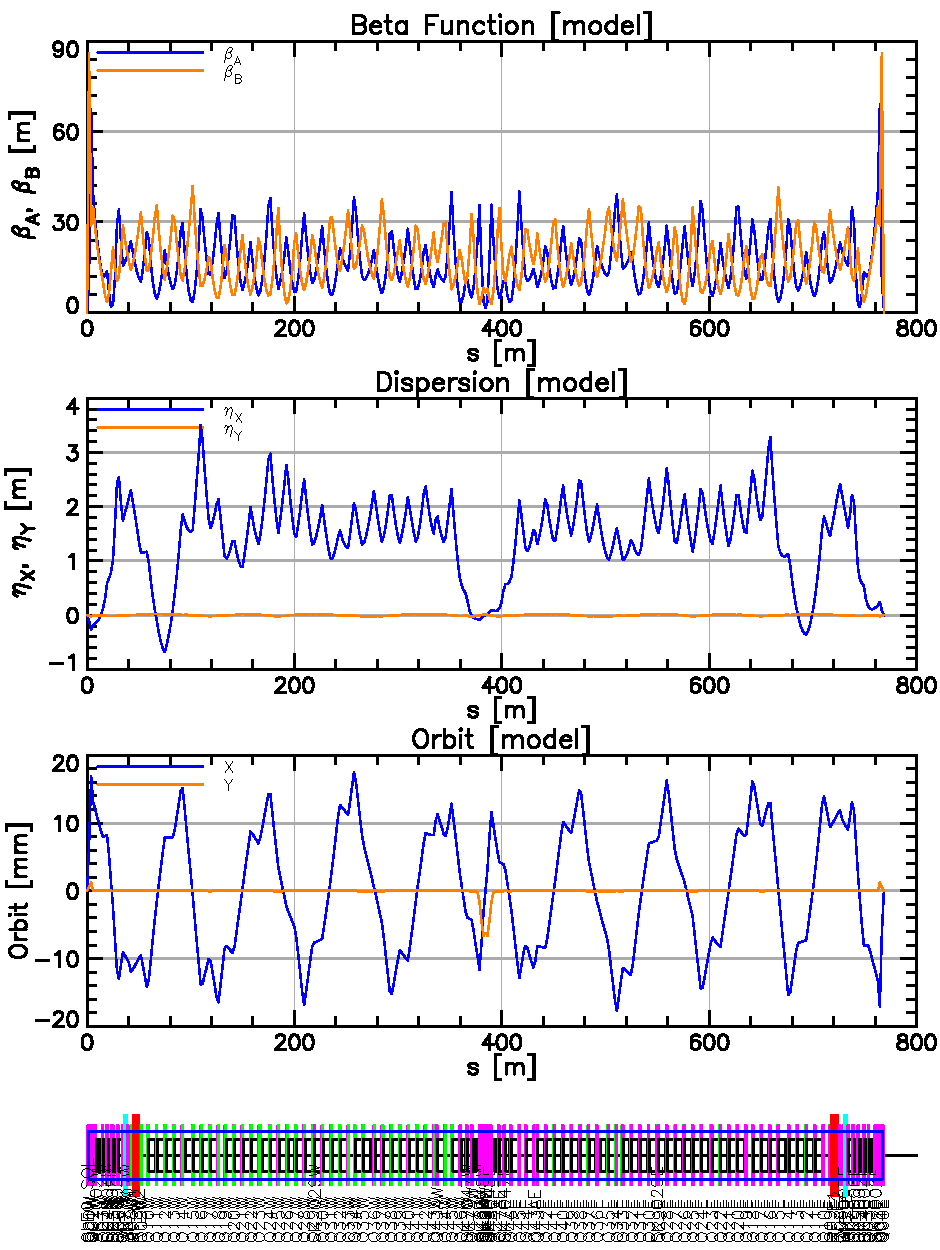
\includegraphics[width=2.5in]{tao-start.pdf}
\hfil
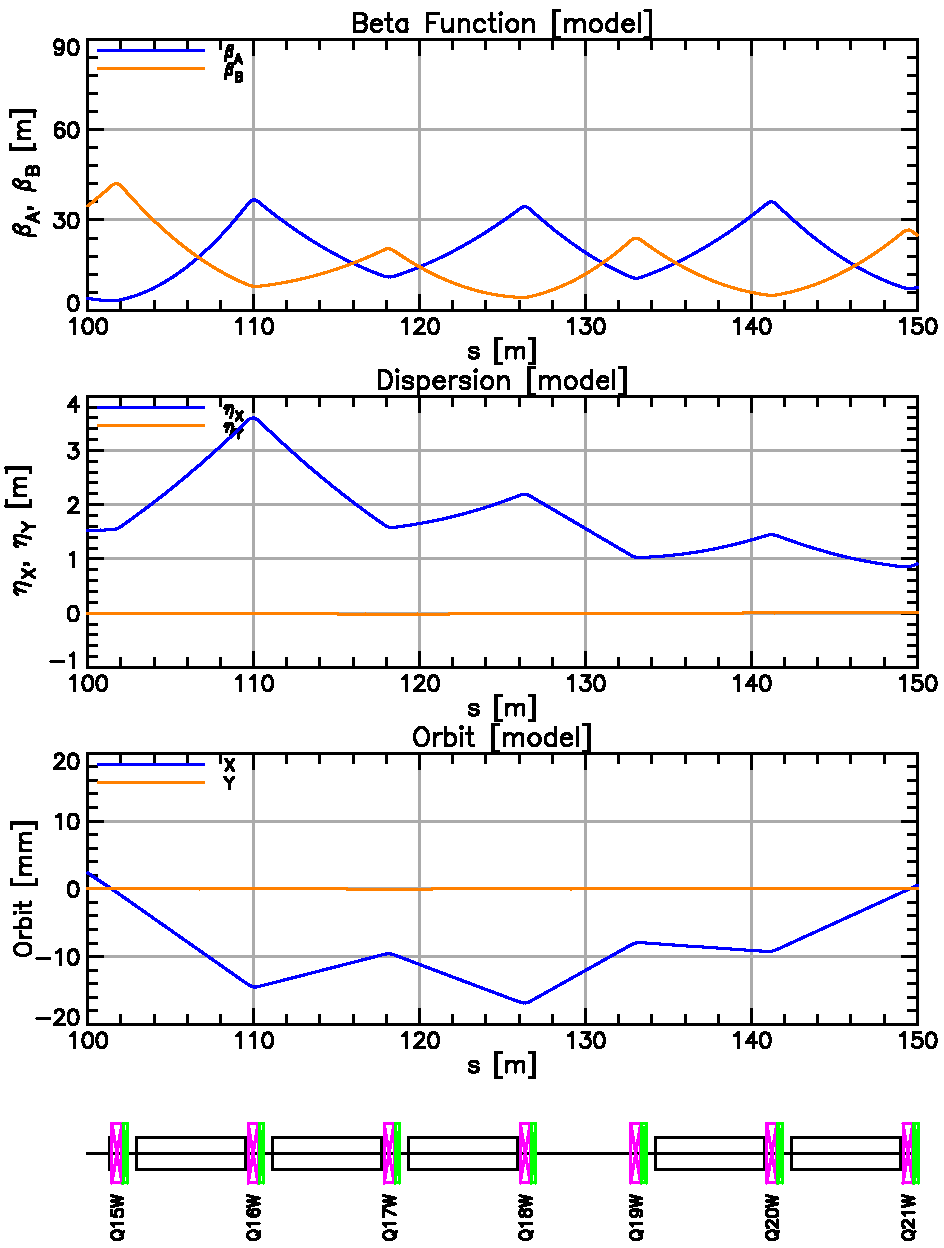
\includegraphics[width=2.5in]{tao-x-scale.pdf}
\caption{Left: Initial \tao plot window with the bmad_L9A18A000-_MOVEREC.lat lattice.
Right: Plot window after horizontal scaling.}
\label{f:tao-start}
\end{centering}
\end{figure}

If all goes well, when \tao is started a plotting window will pop up. For the example given
in \sref{s:starting.tao}, this window will looks as shown on the left in
\fig{f:tao-start}. If the plot window is too large (or too small), the \vn{-geometry} option
can be used at startup to specify the window size. For example:
\begin{display}
  \$ACC_ROOT_DIR/production/bin/tao -geometry 300x500 -lat ....
\end{display}
With this example, \tao would open a plotting window 300 pixels wide by 500 pixels tall.
To prevent any plotting, use the \vn{-noplot} option.

The plot can be scaled vertically using the \vn{scale} command. To scale the plot horizontally, 
the command \vn{x_scale} is used. Thus, to scale all the plots horizontally in our present example use
the command
\begin{display}
  \BF{Tao> x_sca all 100 150}
\end{display}
This scales all the horizontal scale to go from 100~meters to 150~meters. This gives the
right plot in Fig.~\ref{f:tao-start}.

The \vn{show plot} command will give some details on plotting:
\begin{display}
  \BF{Tao> show plot}

    plot_page parameters:
    %size                         =      500     600
    %n_curve_pts                  =      401
    %text_height                  = 12.000
    %main_title_text_scale        = 1.300
    ... ETC., ETC ...

  Templates:
     Plot                  .Graph   Description
     --------------------  -------- -------------------
     alpha                 .g       Twiss alpha function
     b_div_curl            .g       Magnetic Field Divergence and Curl along orbit
     b_field               .g       Magnetic Field Along Orbit
     beta                  .g       Twiss beta function
     cbar                  .g       Cbar coupling matrix
     dbeta                 .g       Chromatic normalized beta beat
     deta                  .g       Second order dispersion
     detap                 .g       Second order dispersion slope
     dphi                  .g       Chromatic phase deviation
     dynamic_aperture      .g       Dynamic aperture using universe calc
    ... ETC., ETC ...

                                                 Location on Page
  Plot Region         <-->  Plot                 x1    x2    y1    y2
  -----------               -----------------------------------------
  layout              <-->  lat_layout          0.00  1.00  0.00  0.15
  r11                 <-->                      0.00  1.00  0.15  1.00
  r12                 <-->                      0.00  1.00  0.58  1.00
  r22                 <-->                      0.00  1.00  0.15  0.58
  r13                 <-->  beta                0.00  1.00  0.72  1.00
  r23                 <-->  dispersion          0.00  1.00  0.43  0.72
  r33                 <-->  orbit               0.00  1.00  0.15  0.43
    ... ETC., ETC ...
\end{display}
Essentially, the plot window is divided into \vn{regions}. By default (without any
initialization file (\sref{s:tao.init})), these regions have names like \vn{r13},
\vn{r22}, etc. By default, the \vn{beta} plot, for example, is placed in the \vn{r13}
region and the \vn{r13} regions inhabits roughly the top of third of the plot window. 

To change what plots are displayed, use the \vn{place} command:
\begin{display}
  \BF{Tao> place r23 energy  ! Put an energy plot in the r23 region}
\end{display}
To clear a particular plot from the screen, place \vn{none} in that region
\begin{display}
  \BF{Tao> place * none}
\end{display}
the star, \vn{*}, refers to all regions so the above command clears the entire plot
display.

One useful plot is the \vn{floor_plan} plot which displays the placement of the elements.
An example of this is shown in Fig.~\ref{f:floor.plan}.

\begin{figure}
  \centering
  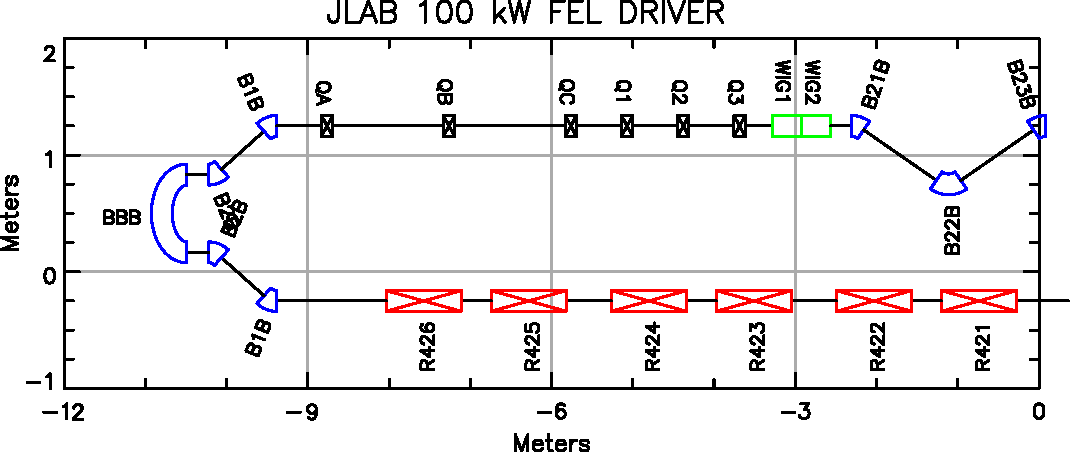
\includegraphics[width=4in]{floor-plan.pdf}
  \caption{Example Floor Plan drawing.}
  \label{f:floor.plan}
\end{figure}

See the \vn{Plotting} chapter in the \tao manual as well as the \vn{Initializing
Plotting} section of the \vn{Tao Initialization} chapter for more details. 

%------------------------------------------------------------------------------
\section{Tao Initialization Files}
\label{s:tao.init}

\tao initialization files are used to customize plotting, define variables and data used
in nonlinear optimization, setup beam parameters for tracking of beams, etc. [Beams in
\tao are used for simulating such things as the effect of coherent synchrotron radiation.]

Example initialization files can be found in the \vn{tao/examples} directory. Information
on the syntax of initialization files can be found in the \vn{Tao Initialization} chapter
in the \vn{tao} manual.

%------------------------------------------------------------------------------
\section{Types of lattices in Tao}

There are three types of lattices in Tao:
  \begin{description}
  \item[Design Lattice] \Newline 
The \vn{design} lattice corresponds to the lattice read in from the lattice description
file(s). In many instances, this is the particular lattice that one wants the actual
physical machine to conform to. The \vn{design} lattice is fixed. Nothing is allowed to
vary in this lattice.
  \item[Model Lattice] \Newline
Except for some commands that explicitly set the \vn{base} lattice, all \tao commands to
vary lattice variables vary quantities in the \vn{model} lattice. Notice that in
Fig.~\ref{f:tao-start} it is the \vn{model} lattice that is being plotted.
  \item[Base Lattice] \Newline
It is sometimes convenient to designate a reference lattice so that changes in the
\vn{model} from the reference point can be examined.  This reference lattice is called the
\vn{base} lattice.
  \end{description}
Initially when starting \tao the three lattices, \vn{design}, \vn{model}, and \vn{base}
are the same.

%------------------------------------------------------------------------------
\section{Tao Universe}

In \tao, a \vn{universe} is a \vn{design}, a \vn{model}, and a \vn{base} lattice, along
with associated data. \tao can handle Multiple universes. For example, \tao could be setup
so that the data associated with a universe could be from an orbit measurement with
different universes having data from different orbit measurements where the settings of
the steerings in the machine are different for each orbit. This can be used, therefore,
for orbit response matrix (ORM) analysis.

Multiple universes may only be created using a \tao initialization file (\sref{s:tao.init}).

%------------------------------------------------------------------------------
\section{Tao Show Universe Command}

The \tao \vn{show universe} command in \tao shows information about the lattice:
\begin{display}
  \BF{Tao> show uni} 
  Universe:        1
  Branch:          0
  %n_d2_data_used        =        0
  %n_data_used           =        0
  ETC. ETC...

  Lattice name:           L9A18A000-_MOVEREC
  Used line in lat file:  CESR
  Lattice file name:      tao/examples/cesr/bmad_L9A18A.bmad
  Reference species:      Electron
  Reference energy:         5.28900000E+09
  ETC. ETC...
                        X          |            Y
                 Model     Design  |     Model     Design
          Q     10.530     10.530        9.578      9.578  ! Tune
      Chrom     -1.168     -1.168       -0.936     -0.936  ! dQ/(dE/E)
     J_damp      1.011      1.011        1.006      1.006  ! Damping Partition
  Emittance  2.033E-07  2.033E-07    1.791E-11  1.791E-11  ! Meters
  ETC. ETC...

                   Model     Design
      Z_tune:     0.0000     0.0517   ! design value calculated with RF on
     Sig_E/E:  6.759E-04  6.759E-04
 Energy Loss:  1.150E+06  1.150E+06   ! Energy_Loss (eV / Turn)
      J_damp:  1.983E+00  1.983E+00   ! Longitudinal Damping Partition #
  Alpha_damp:  2.157E-04  2.157E-04   ! Longitudinal Damping per turn
  ETC. ETC...
\end{display}

%------------------------------------------------------------------------------
\section{Tao Show Global Command}

The \tao \vn{show global} command shows information about global parameters:
\begin{display}
  \BF{Tao> show global}
  Global parameters:
    %bunch_to_plot                 =        1
    %label_lattice_elements        = T
    %label_keys                    = T
    %phase_units                   = Radians
    %beam_timer_on                 = F
    %command_file_print_on         = T
    %disable_smooth_line_calc      = F
    %lattice_calc_on               = T
    %plot_on                       = F
    %rf_on                         = F
    %wait_for_CR_in_single_mode    = F
    %prompt_string                 = Tao
    ETC., ETC...
\end{display}

%------------------------------------------------------------------------------
\section{Tao Show Lattice Command}

The \tao \vn{show lattice} command shows element-by-element parameters such at Twiss
parameters, etc.:
\begin{display}
  \BF{Tao> show lattice 1:6}
      Values at End of Element:
  Ix  name          key             s       l    beta     phi    eta ...
                                                    a       a      a ...
   1  IP_L0         MARKER      0.000   0.000    0.95   0.000  -0.00 ...
   2  CLEO_SOL#3    SOLENOID    0.622   0.622    1.34   0.582  -0.02 ...
   3  DET_00W       MARKER      0.622   0.000    1.34   0.582  -0.02 ...
   4  CLEO_SOL#4    SOLENOID    0.638   0.016    1.37   0.593  -0.02 ...
   5  Q00W#1        QUADRUPOLE  2.163   0.408   15.96   1.045  -0.13 ...
   6  D003          DRIFT       2.493   0.331   27.03   1.061  -0.17 ...
  Ix  name          key             s       l    beta     phi    eta ...
                                                    a       a      a ...
\end{display}

There are many options that can be used with the \vn{show lattice} command:
\begin{display}
  \BF{Tao> help show lat}
  Syntax:           
    show lattice {-0undef} {-all} {-attribute <attrib>} {-base}
        {-blank_replacement <string>}  {-branch <name_or_index>}
        {-custom <file_name>} {-design} {-floor_coords} {-lords} {-middle}
        {-no_label_lines} {-no_tail_lines} {-no_slaves} {-orbit} {-radiation_integrals}
        {-remove_line_if_zero <column #>} {-s <s1>:<s2>} {-tracking_elements}          
        {<element_list>}

  Show a table of Twiss and orbit data, etc. at the specified
  element locations. The default is to show the parameters at the exit
  ETC., ETC...
\end{display}
The \vn{-floor_coords} option displays the global floor coordinates of the elements,
the \vn{-radiation_integrals} option displays radiation integrals for the lattice elements,
the \vn{-custom} option allows the user to construct a custom table, etc., etc. 

%------------------------------------------------------------------------------
\section{Tao Show Element Command}

The \tao \vn{show element} command shows information about a given lattice element:

\begin{display}
  \BF{Tao> show ele q10w}
   Element #               90
   Element Name: Q10W
   Element Type: "CSR QUAD CUR  10"
   Element Alias: "Q10W"
   Key: Quadrupole
   S:             58.654999
   Ref_time:  1.956520E-07

   Attribute values [Only non-zero/non-default values shown]:
       1   L                            =  6.0000000E-01
       4   K1                           =  2.6512600E-01
      13   SPIN_FRINGE_ON               =  T (1)
      31   L_HARD_EDGE                  =  6.0000000E-01
      46   B1_GRADIENT                  = -4.6774072E+00
      50   DELTA_REF_TIME               =  2.0013846E-09
  ETC., ETC...
\end{display}

There are many options that can be used with the \vn{show element} command:
\begin{display}
  \BF{Tao> help show element}
  Syntax:
    show element {-attributes} {-base} {-data} {-design} {-all} {-field}
        {-floor_coords} {-no_slaves} {-ptc} {-taylor} {-wall} {-xfer_mat} <ele_name>

  This shows information on lattice elements. The syntax for "<ele_name>"
  is explained in section . If "<ele_name>" contains a wild card or a
  ETC., ETC...
\end{display}
For brevity's sake The default output from the \vn{show element} command attempts
to only show the most useful information. Use the options of the \vn{show element}
command to taylor what is output. In particular, the \vn{-all} option will show 
be on the verbose side.

Wild card characters may be used with the \vn{show element} command. In this case
a list of matching elements will be printed:
\begin{display}
  \BF{Tao> show ele sbend::b0*}
          22  B03W                                            11.949
          24  B03AW                                           13.970
          30  B04W                                            18.653
          38  B05W                                            23.698
          46  B06W                                            28.743
          54  B07W                                            33.789
         816  B07E                                           737.876
         824  B06E                                           742.921
         832  B05E                                           747.966
         840  B04E                                           753.012
         846  B03AE                                          756.100
         848  B03E                                           759.423
  Number of Matches: 12
\end{display}
This example shows all lattice elements that are \vn{sbend} elements whose name begins
with \vn{b0}.

%------------------------------------------------------------------------------
\section{Modifying Parameters in Tao}

The \vn{change} and \vn{set} commands are used to modify parameters in \tao.  Generally,
the \vn{change} command is used to vary real valued parameters while \vn{set} is used
for any type of attribute.

With the \vn{change} command, change values can either be deltas from the current value,
absolute values (using a \vn{@} prefix), or offsets from the design value (using a \vn{d}
prefix) Examples:
\begin{display}
  \BF{Tao> change ele q* 1e-4}
\end{display}
This changes all elements whose name begins with \vn{q} by an amount 1e-4.
\begin{display}
  \BF{Tao> change beam_start x @0.001}
\end{display}
This sets the $x$ starting position of a beam or particle being tracked to 0.001
\begin{display}
  \BF{Tao> change variable steering[34] d 1e-4}
\end{display}
This sets the variable named \vn{steering[34]} (variables are defined by the user via a
\tao initialization file) to the design value (the value as given in the design lattice)
plus 1e-4.

The \vn{set} command can set many things:
\begin{display}
  \BF{Tao> help set}
  The "set" command is used to set values for data,
  variables, etc. Format:
    set beam_init {n@}<component> = <value>             
    set bmad_com <component> = <value>                  
    set csr_param <component> = <value>                 
    set curve <curve> <component> = <value>             
    set data <data_name>|<component> = <value>          
    set default <parameter> = <value>                   
    set element <element_list> <attribute> = <value>    
    set floor_plan <component> = <value>                
    set geodesic_lm <component> = <value>               
    set global <component> = <value>                    
    set graph <graph> <component> = <value>             
    set key <key> = <command>                           
    set lat_layout <component> = <value>                
    set lattice {n@}<destination_lat> = <source_lat>    
    set opti_de_param <component> = <value>             
    set plot <plot> <component> = <value>               
    set plot_page <component> = <value1> {<value2>}     
    set ran_state = <random_number_generator_state>     
    set universe <what_universe> <on/off>               
    set universe <what_universe> recalculate            
    set universe <what_universe> mat6_recalc <on/off>   
    set universe <what_universe> track_recalc <on/off>  
    set variable <var_name>|<component> = <value>       
    set wave <component> = <value>                      
  ETC., ETC...
\end{display}

%------------------------------------------------------------------------------
\section{Lattice Optimization in Tao}

Lattice optimization includes such things as designing lattices and flattening orbits.
The basic idea is to define, via a \tao initialization file, the parameters to be varied
and the merit function to be minimized. Once that is done, \tao has several optimization
schemes that can be used. The interested read is referred to the \tao manual for the
details.

%------------------------------------------------------------------------------
\section{Customizing Tao}

Besides the customization that can be done via \tao input files, \tao custom code
can be linked with \tao to extend \tao capabilities. For example, custom code can
be used to interface between \tao and an accelerator. In this way \tao can be used
as an online model to, for example, read orbit data, calculate via optimization corrector
strengths, and then load the calculated corrector changes back into the machine.

For more details on using custom code with \tao, see the \vn{Customizing Tao} chapter
in the \tao manual.

%------------------------------------------------------------------------------
\Section{Creating Your Own Bmad Based Programs}

At some point you might want to start creating you own programs. Documentation for this is
at:
\begin{display}
  \url{https://wiki.classe.cornell.edu/ACC/ACL/BuildSystem}
\end{display}
Programming with \bmad is also discussed in detail in the \bmad manual. The \vn{examples} directory
holds a set of example programs that can be used for templates.

As a simple example, consider setting things up to compile the simple bmad program
discussed in the \vn{Introduction to Bmad Programming} chapter of the \bmad manual.
The program code and lattice input file is in the directory:
\begin{display}
  \BF{\$ACC_ROOT_DIR/examples/simple_bmad_program/}
\end{display}

The first thing to do is to create a \vn{base} directory for your code and executables. This
directory will be named \vn{base_dir} in this example but you can name it anything you
want. Important: Do not create \vn{base_dir} within a \vn{Distribution} tree. Keeping things
separate greatly simplifies maintenance.

After you have created \vn{base_dir}, cd to that directory. Now copy the
simple_bmad_program directory to a new directory called \vn{base_dir/my_prog_dir}:
\begin{display}
  \BF{base_dir> cp -r \$ACC_ROOT_DIR/examples/simple_bmad_program/ my_prog_dir}
  \BF{base_dir> cd my_prog_dir}
  \BF{my_prog_dir> ls}

  lat.bmad   layout.bmad   simple_bmad_program.f90
\end{display}

The \vn{my_prog_dir} directory has the program code and lattice files but is
missing the \vn{cmake} scripts for compiling and linking the program.  [\vn{cmake} is the
open-source tool used to compile \bmad.] The scripts used by the \vn{Distribution} or
\vn{Release} for compiling are structured for a different directory organization so they
are not appropriate here. Rather, the ``template'' scripts in
examples/cmake_template_scripts work well so copy them into the my_prog_dir
directory:
\begin{display}
  \BF{my_prog_dir> cp \$ACC_ROOT_DIR/examples/cmake_template_scripts/* .}
  \BF{my_prog_dir> ls}

  CMakeLists.txt  cmake.test  lat.bmad  layout.bmad simple_bmad_program.f90
\end{display}

The scripts are setup to create an executable:
\begin{display}
  \BF{base_dir/production/bin/test}
\end{display}
If you don't like the name \vn{test} then this can be changed by editing the
\vn{cmake.test} file and changing \vn{EXENAME}. In any case, to create the executable,
make sure you are still in the my_prog_dir directory and issue the \vn{mk} command:
\begin{display}
  \BF{my_prog_dir> mk}
\end{display}

After the \vn{mk} command is finished there should be an executable at
\vn{base_dir/production/bin/test}. There will also be a \vn{my_prog_dir/production}
directory that holds intermediate compiled files which can be used in the future to save
compile time when there are multiple code files but not all of them have to be recompiled.
There is nothing in the \vn{my_prog_dir/production} of interest so it can be ignored.

Now you can run the program. While still in the \vn{my_prog_dir} directory (since the
program will look for the lattice file in the default directory), run the program:
\begin{display}
  \BF{../production/bin/test}
\end{display}
The result:
\begin{display}
  [INFO] bmad_parser:
      Parsing lattice file(s). This might take a minute or so...
  [INFO] bmad_parser:
      Created new digested file
    Ix  Name              Ele_type                   S      Beta_a
     0  BEGINNING         BEGINNING_ELE             0.0000      0.9379
     1  IP_L0             MARKER                    0.0000      0.9379
     2  CLEO_SOL#3        SOLENOID                  0.6223      1.3472
     3  DET_00W           MARKER                    0.6223      1.3472
     4  CLEO_SOL#4        SOLENOID                  0.6380      1.3682
     5  Q00W\\CLEO_SOL     SOL_QUAD                  1.7550      8.0285
     6  Q00W#1            QUADRUPOLE                2.1628     16.8607
     7  D003              DRIFT                     2.4934     28.5769
     8  DET_01W           MARKER                    2.4934     28.5769
     9  D004              DRIFT                     2.9240     48.4524
    10  Q01W              QUADRUPOLE                3.8740     66.8800
   
   !---------------------------------------------------------
   ! Information on element: CLEO_SOL
   
    Element #              872
    Element Name: CLEO_SOL
    Key: Solenoid
    S:              1.755000
    Ref_time:  5.854050E-09
   
    Attribute values [Only non-zero/non-default values shown]:
        1   L                            =  3.5100000E+00
        5   KS                           = -8.4023386E-02
       13   SPIN_FRINGE_ON               =  T (1)
       31   L_HARD_EDGE                  =  3.5100000E+00
       49   BS_FIELD                     = -1.4823578E+00
  ... etc., etc...
\end{display}

\end{document}
